\documentclass{article}
\usepackage[english]{babel}
\usepackage{listings}
\usepackage{xcolor}
\definecolor{light-gray}{gray}{0.95}
\newcommand{\code}[1]{\colorbox{light-gray}{\texttt{#1}}}

% Set page size and margins
% Replace `letterpaper' with `a4paper' for UK/EU standard size
\usepackage[letterpaper,top=2cm,bottom=2cm,left=3cm,right=3cm,marginparwidth=1.75cm]{geometry}
\usepackage[most]{tcolorbox}

\newtcolorbox{mybox}{
enhanced,
boxrule=0pt,frame hidden,
borderline west={4pt}{0pt}{green!75!black},
colback=green!10!white,
sharp corners
}
% Useful packages
\usepackage{amsmath}
\usepackage{graphicx, tcolorbox}
\usepackage[colorlinks=true, allcolors=blue]{hyperref}
\usepackage{xcolor}
\usepackage[dvipsnames]{xcolor}

\title{PyTorch}
\author{SS}

\begin{document}
\maketitle

\begin{abstract}
QnA on PyTorch, NN.
\end{abstract}

\section{QnA}
% 
%*********************************************************************
%*********************************************************************
\noindent
{\color{red} \rule{\linewidth}{0.5mm}}
\textcolor{red}{Name some different components of PyTorch} \\
\noindent
{\color{red} \rule{\linewidth}{0.5mm}}

\begin{itemize}
\color{blue}
\item \textbf{Tensors}: Tensors are very homogeneous to the Numpy array and it is also multi-dimensional. The tensors are accessible in PyTorch as a "torch" e.g. torch.CharTen, torch.intTesnor, torch.FloatTensor
\item \textbf{Variable}: \textit{A variable works as a wrapper around the Tensor to clutch the gradient.} You can find variables under the "torch.autograd" in the form of torch autograd variable.
\item \textbf{Parameters}: The work of a parameter is to wrap the variable and we use it when the Tensors of a module do not possess a gradient. We can find parameters under the toch.nn in the form of torch.nn Parameter.
\item \textbf{Functions}: Functions do not posess any memory and their work is to transform the operations. Some examples of functions are torch.sum, torch.log etc. Functions are implemented using torch.nn.functional
\item \textbf{Modules}: Modules are the base calls of all neural networks and they also can contain different functions, modules, and parameters. It is efficient in storing learnable weights and states. Modules can be applied as torch.nn.Linear, torch.nn.Conv2d etc.
\end{itemize}
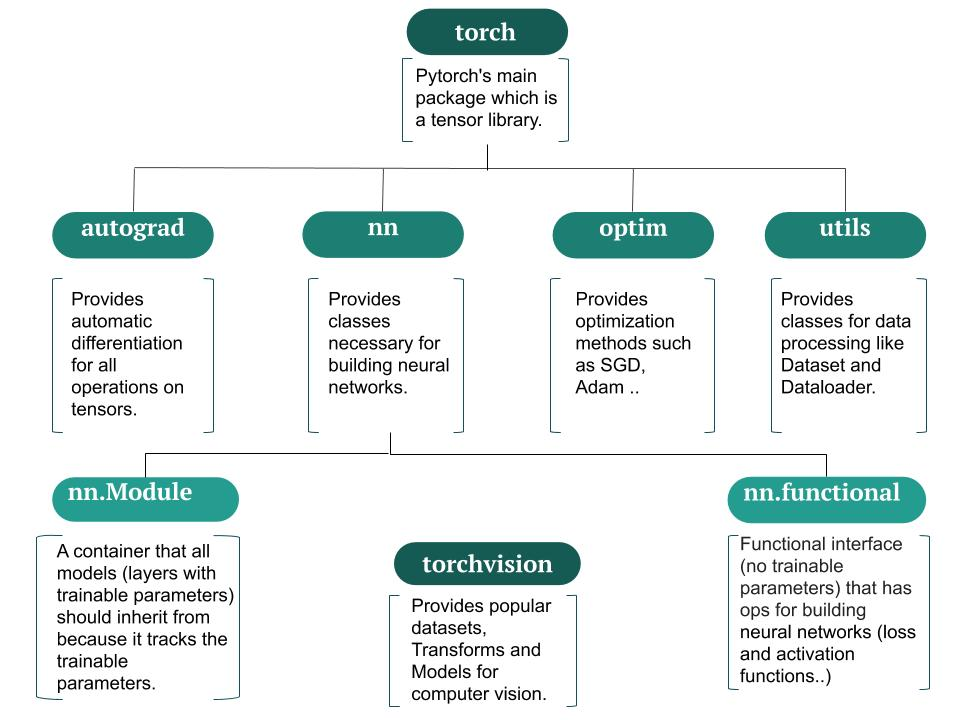
\includegraphics[width=5cm, height=3.5cm]{LSTM/images/Pytorch-package-hierarchy.jpg}

\\

%*********************************************************************
%*********************************************************************
\noindent
{\color{red} \rule{\linewidth}{0.5mm}}
\textcolor{red}{What are different layers available in torch.nn? Explain with examples} \\
\noindent
%                      
%*********************************************************************
\noindent
{\color{red} \rule{\linewidth}{0.5mm}}
\textcolor{red}{What are some methods to reshape the tensor dimension in PyTorch?} \\
\noindent
{\color{red} \rule{\linewidth}{0.5mm}}
There are multiple methods to reshape tensor dimensions in PyTorch, some of which are:
\begin{itemize}
    \item torch.reshape(input, shape): Reshapes input to shape (if compatible)
    \item torch.Tensor.view(shape): Returns a view of the original tensor in a different shape but shares the same data as the original tensor.
    \item torch.permute (input, dims): Returns a view of the original input with a dimensions rearranged to dims.
\end{itemize}

%*********************************************************************
%                      deactivate a Virtual Environment
%*********************************************************************
\noindent
{\color{red} \rule{\linewidth}{0.5mm}}
\textcolor{red}{What are the fundamental steps of a training loop in PyTorch?} \\
\noindent
{\color{red} \rule{\linewidth}{0.5mm}}
In a typical training loop, the following operations are implemented for each batch during each epoch:
\begin{itemize}
    \item Get a batch of training data
    \item Zero the optimizer gradient
    \item Perform the \textit{inference} - that is, get predictions from the model for an input batch
    \item Calculate the loss for that set of predictions from the model for an input batch
    \item Calculate the backward gradients over the learning weights
    \item Adjust the model learning weights based on the observed gradients for this batch, according top the optimizer algorithm we choose
    \item Store the loss for each training step to be used later for reporting
\end{itemize}
\begin{lstlisting}[language=Python]
running_loss = 0
for i, data in enumerate(training_batch_set):
    #1 Every data instance is an input + label pair
    inputs, labels = data
    #2 Zero your gradients for every batch
    optimizer.zero_grad()
    #3 Make predictions for this batch
    outputs = model(inputs)
    #4 complute the loss
    loss = loss_fn(outputs, labels)
    #5 Compute the loss gradients
    loss.backward()
    #6 Adjust Learning weights
    optimizer.step()
    #7 Gather Data for Reporting
    running_loss += loss.item()
\end{lstlisting}
%*********************************************************************
%                      Loss Function vs Optimizer
%*********************************************************************
\noindent
{\color{red} \rule{\linewidth}{0.5mm}}
\textcolor{red}{What is the difference between Loss Function and Optimizer?} \\
\noindent
{\color{red} \rule{\linewidth}{0.5mm}}
The loss function is the quantity that will be minimized during training. The optimizer determines how the network will be updated based on the loss function. \\
Optimizers play a pivotal role in guiding gradient-based optimization algorithms. They drive the learning process by adjusting model weights based on computed gradients. In PyTorch, optimizers such as SGD and its variants, such as Adam and RMSprop, are readily available.
\begin{itemize}
    \item SGD: Often used as a baseline for optimization. Adjusts weights proportionally to the average negative gradient
    \item Adam: Adaptive and combines aspects of RMSprop and momentum. Often a top choice for tasks across domains
    \item Adagrad: Adjusts learning rate for each parameter
    \item RMSprop: Adaptive in nature and modifies learning rates based on moving averages
    \item Adadelta: Similar to Adagrad but aims to alleviate its learning rate decay drawback
    \item AdamW
    \item Sparse Adam
    \item ASGD: Averaged SGD
    \item Rprop
    \item LBFGS: Particularly useful for small datasets due to numerically computing the Hessian matrix.
\end{itemize}

%*********************************************************************
%                     Requirements.txt
%*********************************************************************
\noindent
{\color{red} \rule{\linewidth}{0.5mm}}
\textcolor{red}{Explain Batch Normalization and its effects on training convergence} \\
\noindent
{\color{red} \rule{\linewidth}{0.5mm}}
Batch Normalization (BN) is a pivotal technique for training deep neural networks. It operates by standardizing activations within each mini-batch, which confers several advantages.\\
Benefits of Batch Normalization:
\begin{itemize}
    \item Mitigates Vanishing/Exploding Gradients: By normalizing inputs, BN ensures steady learning rate, preventing extremes that impede training
    \item Facilitates Smoother Loss Landscape: Normalizing mini-batch activation renders optimization more roll out, making it easier for the model to converge 
    \item Acts as a Regularizer: Though not its designed function, BN introduces noise during training similar to Dropout, which can curb overfitting
    \item Maintains Model Stability: BN lessens the dependence of model parameters on the initial value and reduces the likelihood of parameters diverging
\end{itemize}
%*********************************************************************
\noindent
{\color{red} \rule{\linewidth}{0.5mm}}
\textcolor{red}{How batch normalization enables faster convergence?} \\
\noindent
{\color{red} \rule{\linewidth}{0.5mm}}

\begin{itemize}
    \item Batch Neutrality: For each mini-batch, BN centers and scales the data. However, it does not alter the data from past pr future batches. This constraint can speed up the learning process.
    \item Improved Gradient Flow: BN focuses on standardizing activators to facilitate a consistent gradient flow during backpropagation, addressing issues like vanishing and exploding gradients. 
    \item Role in Weight Initialization: BN can assist in maintaining activation distributions, weight initialization methods like Xavier and He.
    \item Decoupling from Learning Rate Selection: Although BN is sensitive to learning rates, it's less dependent on specific learning rate value
    \item Application Dynamics: BN is optimized for training rather than inference and brings pronounced benefits in accurate estimates post training.
\end{itemize}
%*********************************************************************
\begin{lstlisting}[language=Python]
import torch
import torch.nn as nn
import torch.optim as optim
# Create a simple NN
class Net(nn.Module):
    def __init__(self):
        super(Net, self).__init__()
        self.fc1 = nn.Linear(28*28, 300)
        self.bn1 = nn.BatchNorm1d(300) # Batch Norm Layer
        self.fc2 = nn.Linear(300,10)
        self.bn2 = nn.BatchNorm1d(10) # Batch Norm Layer
    def forward(self, x):
        x = x.view(-1, 28*28) # Flatten the input
        x = self.fc1(x)
        x = self.bn1(x) # Apply Batch Normalization
        x = torch.relu(x)
        x = self.fc2(x)
        x = self.bn2(x) # Batch Normalization
        return x
# Initialize the network and the dataset
net = Net()
optimizer = optim.SGD(net.parameters(), lr = 0.01)
criterion = nn.CrossEntropyLoss()
# Inside the training loop
for inputs, target in dataloader:
    optimzer.zero_grad()
    outputs = net(inputs)
    loss = criterion(outputs, targets)
    loss.backward()
    optimizer.step()
\end{lstlisting}
Different types of Normalizations:
\begin{itemize}
    \item Batch Norm
    \item Layer Norm
    \item Instance Norm
    \item Group Norm
\end{itemize}
%*********************************************************************
\section{Time Series Data}
%*********************************************************************
\noindent
{\color{red} \rule{\linewidth}{0.5mm}}
\textcolor{red}{How do you manage and preprocess time-series data in PyTorch for RNNs?} \\
\noindent
{\color{red} \rule{\linewidth}{0.5mm}}
Time-Series data presents unique challenges for RNNs due to its sequential nature. Leveraging such data in PyTorch involves several key steps, from dataset creation to model training.
\subsection{Dataset Creation}
\subsubsection{Data Slicing}
Divide your time-series data into $(X,y)$ pairs, where $X$ is the input window and $y$ is the target. This step often involves creating a sliding or expanding window over the time series.
\subsubsection{Tensor Transformation}
Convert your data to PyTorch tensors, and, if applicable the right data type using .float(), .long(), or other casting methods as necessary.
\subsubsection{Data Loader Setup}
Use PyTorch's DataLoader to batch, shuffle and potentially \textit{parallelize} your data.
\begin{lstlisting}[language=Python]
import torch
import torch.utils.data
import Dataset
import DataLoader

class TimeSeriesDataset(Dataset):
    def __init__(self, data, input_window=10, target_window=1):
        self.data = torch.FloatTensor(data)
        self.input_window = input_window
        self.target_window = target_window

    def __len__(self):
        return len(self.data) - self.input_window - self.target_window + 1

    def __getitem__(self, idx):
        input_start = idx
        input_end =  idx + self.input_window
        target_start = input_end
        target_end = input_end + self.target_window

        x = self.data[input_start:input_end]
        y = self.data[target_start:target_end]

        return x,y

data = range(100) # Actual Time Series Data (Replace)

dataset = TimeSeriesDataset(data)
dataloader = DataLoader(dataset, batch_size=32, shuffle=True)
\end{lstlisting}
\subsection{Model Input Requirements}
PyTorch's RNN module expects inputs to be 3D Tensors with dimensions: Batch Size, Sequence Length, and Input Size.
\subsubsection{Batch Size}
Represents the number of sequences in a batch
\subsubsection{Sequence Length}
Corresponds to the length of each sequence
\subsubsection{Input Size}
Denotes the number of features at each time step.
\subsection{Data Standardization}
\begin{itemize}
    \item Calculate statistics
    \item Standardization
    
\end{itemize}
\begin{lstlisting}[language=Python]
mean = data.mean()
std = data.std()
standardized_data = (data-mean)std
\end{lstlisting}
\subsection{Handling Variable Length Sequence}
Employing RNNs for datasets with variable length sequences requires additional steps:
\subsection{Sequence Padding}
Bring all sequences to the same length by padding shorter ones with a designated padding value. PyTorch offers a ready-to-use function for this.
\subsubsection{Sequence Sorting}
For optimized training, sort sequences in descending order based on their lengths, and keep track of the original indices for restoring the order later during evaluation.
%*********************************************************************
\noindent
{\color{red} \rule{\linewidth}{0.5mm}}
\textcolor{red}{What is the difference between Input Size and Hidden Size in LSTM?} \\
\noindent
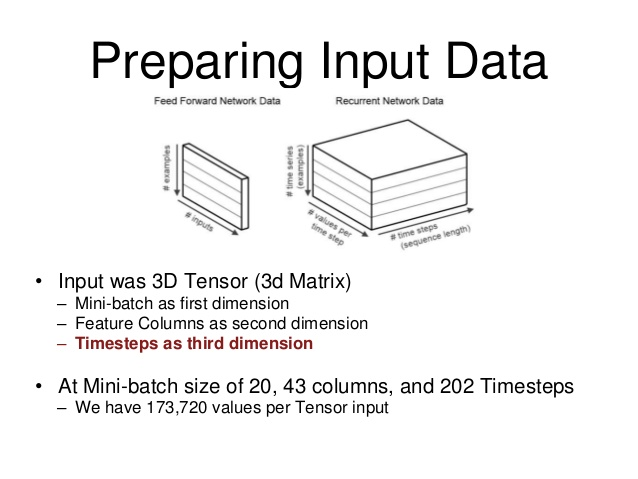
\includegraphics[width=7cm, height=4.5cm]{LSTM/images/InputData.jpg}
%*********************************************************************
\noindent
{\color{red} \rule{\linewidth}{0.5mm}}
\textcolor{red}{What is the difference between Input Size and Sequence Length in LSTM?} \\
\noindent
%*********************************************************************
\section{Data Handling and Preprocessing}
%*********************************************************************
\noindent
{\color{red} \rule{\linewidth}{0.5mm}}
\textcolor{red}{How do you create a data loader in PyTorch for custom datasets?} \\
\noindent
Data loaders in PyTorch enable parallelized loading of large datasets, making it easier to manage data for training and validation.
\subsection{The DataLoader Object}
A Dataloader wraps a dataset and provides the following key functionalities:
\begin{itemize}
    \item Batching Data
    \item Shuffling the data (if necessary)
    \item Loading the data in parallel using \textit{multiprocessing} and \textit{multithreading} in Python
    \item Pinning the memory (for GPU training) using \code{pin\_memory}
    \item Handling the last batch using drop last
\end{itemize}
%*********************************************************************
\subsubsection{Defining a Custom Dataset}
To create a data loader for a custom dataset, you need to extend the \code{torch.utils.data.Dataset} class. This entails implementing the following methods:
\begin{itemize}
    \item \code{\_\_len()\_\_} This method should return the size of the dataset
    \item \code{\_\_getitem\_\_(index)} This method loads and reruns the dataset item at the given index. It is used to retrieve the individual data points and their corresponding labels
\end{itemize}
%*********************************************************************
\subsubsection{Implementing a Custom Dataset}
\begin{lstlisting}[language=Python]
import torch
from torch.utils.data import Dataset, DataLoader
# Define the custom dataset
class CustomDataset(Dataset):
    def __init__(self):
        # Initialize dataset attributes
        pass
    def __len__(self):
        # Return the total number of samples in the dataset
        pass
    def __getitem__(self, index)
        # Implement to load and return sample from the dataset at the given index
        pass
# Initialize the Dataset
dataset = CustomDataset()

# Create a data loader from the dataset
data_loader = DataLoader(dataset, batch_size=64, shuffle=True, num_workers=2)
\end{lstlisting}
The common parameters are:
\begin{itemize}
    \item \code{batch\_size}: Number of sample in each batch of data
    \item \code{shuffle}: Whether to shuffle the dataset
    \item \code{num\_workers}: Number of processes to use for dataloading
\end{itemize}
%*********************************************************************
\subsection{Transforms}
\noindent
{\color{red} \rule{\linewidth}{0.5mm}}
\textcolor{red}{What is the use of transforms in PyTorch's torchvision package?} \\
\noindent
In PyTorch's torchvision package, transforms are a versatile set of tools for images preprocessing, augmentation, and data normalization. They streamline the transformation of input data before sending it to the neural network. 
\subsection{Core Transform Types}
\begin{itemize}
    \item General Transforms: Basic transformations like resizing and cropping
    \item Tensor-specific Transforms: To convert Numpy arrays to PyTorch Tensors and vice versa
    \item Image-only Transforms: These exclusively target images and carry out a multitude of operationsincluding color jittering and PIL image conversion
\end{itemize}
\subsection{Transformation Composability}
You can aggregate multiple transformations into a single pipeline using the composability
\begin{lstlisting}[language=Python]
import torch
import torchvision.transforms as transforms
from torchvision import datasets
# Load a sample image
img = datasets.CIFAR10(root = 'data/', train=True, download=True)[0][0]
# Define a transformation pipeline
transform = transforms.Compose([
    transforms.RandomCrop(32, padding=4),
    transforms.RandomHorizontalFlip(),
    transforms.ToTensor()
])
# Apply the pipeline to the image
transformed_img = transform(img)
# Visualize the transformed image
plt.imshow(transformed_img.permute(1,2,0).numpy()
plt.show()
\end{lstlisting}
%*********************************************************************
% Reference
%*********************************************************************
\section{Reference}
\begin{itemize}
    \item \href{https://www.youtube.com/watch?v=Y21OR1OPC9As}{Tech With Tim}
    \item \href{https://packaging.python.org/en/latest/guides/installing-using-pip-and-virtual-environments/}{Python Versioning in venv}
    \item \href{https://stackoverflow.com/questions/68376749/problems-installing-python-packages-into-a-virtual-environment-in-visual-studio}{py env in vscode}
    \item \href{https://stackoverflow.com/questions/61528500/installing-venv-for-python3-in-wsl-ubuntu}{venvs in wsl}
\end{itemize}
\end{document}